You might be familiar with sequence diagrams, as shown in Figure \ref{seqdiaexp}:
\begin{figure}
\centering
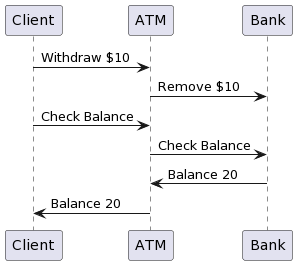
\includegraphics[width=0.5\textwidth]{figures/exampleseq.png}
\caption{\label{seqdiaexp} A sequence diagram example}
\end{figure}
\todo{Give figure of sequence diagram}

Of course, we can define a process that implements such a sequence diagram. In fact, we can define an infinite number of processes that meets such a sequence diagram. Thus, it naturally suggests that what a sequence diagram represents is \textit{not} a process. Rather, it defines a ``type" of a process, something that is usually referred to as a \textbf{protocol}.

Often times, when defining complex systems in the $\pi$-calculus, to see how they interact, we wish to define them against some specific protocol, and thus, we need some method to define such protocols. The mechanism for this is session types.

One last motivation for types: You will find that the syntax for the $\pi$-calculus is actually quite \textit{loose}, in the sense that it defines processes that are ``nonsensical", which is especially true for the higher-order $\pi$-calculus. It's difficult to describe precisely without going into the syntax, so let's make an analogy. Suppose you had some rewriting system that let you define function notation, such as $f(1,2,3)$. The $\pi$-calculus allows you to write equivalents of $f(,)1$, which simply have no meaning. Typing actually prevents such processes from being considered. The typing rules of the $\pi$-calculus are defined such that you can only have well-behaved processes. If this is too abstract, that's fine. It will make more sense as you read through the syntax section.

Based on the latter point of reason, to understand how to write processes requires knowing the typing rules, and so, these rules will be provided in Section \ref{formsyn} as well.

\todo{Might have to rework ...}